\documentclass[article,12pt,onesidea,4paper,english,brazil]{abntex2}

\usepackage{lmodern, indentfirst, nomencl, color, graphicx, microtype, lipsum}			
\usepackage[T1]{fontenc}		
\usepackage[utf8]{inputenc}		

\setlrmarginsandblock{2cm}{2cm}{*}
\setulmarginsandblock{2cm}{2cm}{*}
\checkandfixthelayout

\setlength{\parindent}{1.3cm}
\setlength{\parskip}{0.2cm}

\SingleSpacing

\begin{document}
	
	\selectlanguage{brazil}
	
	\frenchspacing 
	
	\begin{center}
		\LARGE 
		INFORMÁTICA E SOCIEDADE: UMA LEITURA DO PROBLEMA DA EVASÃO ESCOLAR
		
		
		\normalsize
		Italo Jeferson da Silva Brito\footnote{Bolsista PIBIC-EM, italojefersonpvh@gmail.com, Campus Porto Velho Calama.} 
		Xênia de Castro Barbosa\footnote{Orientadora, xênia.castro@ifro.edu.br, Campus Porto Velho Calama.} 
		Gisele Caroline Nascimento dos Santos\footnote{Colaboradora,gisele.santos@ifro.edu.br, Reitoria - IFRO.} 
	
	\end{center}
	
	% resumo em português
	\begin{resumoumacoluna}
		: A evasão escolar apresenta-se como uma questão que tem ganhado visibilidade em diversas pesquisas em educação e tem preocupado muitas instituições de ensino. Nesse sentido, o objetivo deste estudo foi analisar os dados oficiais sobre evasão do Curso Técnico de Informática Integrado ao Ensino Médio do Campus Porto Velho Calama, e os fatores de evasão. O método que deu suporte ao estudo foi o método Histórico (RÜSEN, 2001). Estima-se que os resultados da pesquisa possam contribuir com a reflexão acerca do problema da evasão escolar no IFRO e sensibilizar a gestão para as dificuldades enfrentadas pelos estudantes na permanência e êxito nocurso.
		
		\vspace{\onelineskip}
		
		\noindent
		\textbf{Palavras-chave}: Evasão escolar. Fracasso escolar. Curso Técnico.
	\end{resumoumacoluna}
	
	\section*{Introdução}
	
	A pesquisa foi desenvolvida na modalidade Iniciação Científica Júnior (ICJ), sob a égide do projeto intitulado “Informática e sociedade: um estudo da efetividade do curso técnico de informática do IFRO”, visando identificar os principais fatores que concorrem para a evasão escolar no curso Técnico de Informática Integrado ao Ensino Médio.
	
	As reflexões sobre a problemática histórica da evasão escolar foram feitas com base em Freitag (1980), Frigotto (1989) e Aquino (1997), considerando-se também documentos jurídicos como a Constituição Federal (BRASIL, 1988) e a Lei nº 9.394, de 20 de dezembro de1996.
	
	\section*{Material e Método}
	
O método que deu suporte a este estudo foi método Histórico  (RÜSEN, 2001), que opera com a cultura do tempo presente e documentos diversificados, com vistas a produzir um conhecimento crítico a cercados fenômenos.O método foi selecionado por se mostrar adequado tanto à coleta dos dados, quanto às críticas de ordem hermenêutica e heurística.

O corpus documental do estudo foi composto por relatórios e estatísticas produzidas pelo IFRO e disponibilizadas na ferramenta Painel IFRO, bem como planilhas disponibilizadas pelo Departamento de Assistência ao Educando (DEPAE) do Campus Porto Velho Calama e entrevistas realizadas com 11 estudantes que evadiram do curso Técnico de Informática do Campus Calama entre os anos de 2011 e 2015. Em relação aos dados oficiais, destaca-se que não foi possível  acessar os que tratam da evasão anterior ao ano de 2013 pois de acordo com a instituição os dados referentes a esse ano não estão estruturados, assim os únicos dados anteriores a 2013 de que dispusemos fomos os que nós próprios levantamos com a pesquisa, por meio deentrevistas.

As entrevistas foram realizadas de forma interpessoal e presencial, sempre que possível, e apenas nos casos em que os colaboradores não tiveram tempo para nos receber é que enviamos o roteiro por e-mail. Compreenderam questões abertas e fechadas, possibilitando aos entrevistados informar sobre os fatores que levaram a abandonar o curso.
	
	\section*{Resultados e Discussão}
	
	A evasão escolar, considerada também como fracasso (do estudante, da instituição, das políticas públicas educacionais) é um fator que merece atenção especial no Campus Porto Velho Calama, dado seus números elevados. Em 2014, do total de alunos matriculados quase a metade evadiu, conforme pode ser observado na figura abaixo:
	\begin{figure}[h]
		\centering
		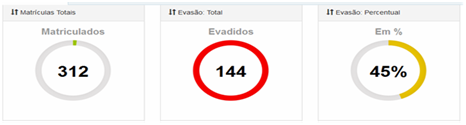
\includegraphics[width=0.7\linewidth]{pip-artigo09-01}
		\caption{Relação Matrículas, evasão e percentual de evasão dos cursos do Campus Calama, 2014}
		\label{fig:pip-artigo09-01}
	\end{figure}
	Esse número elevadíssimo de estudantes que por algum(s) motivo(s) teve de interromper seu processo formativo mostra a relevância do tema a ser discutido e alerta a instituição, a família e o Estado no dever de buscar soluções para esse problema.
	
	O levantamento de dados acerca da evasão escolar por cursos ofertados na unidade de Ensino que constituiu o recorte empírico deste estudo está demonstrado no Quadro a seguir:
	\begin{table}[h]
		\centering
		\caption{Evasão escolar por curso, Campus Porto Velho Calama, 2014}
		\label{my-label}
		\begin{tabular}{ll}
			\hline
			\textbf{Curso}                                             & \textbf{Quantidade} \\
			\hline
			Técnico em Edificações – Ensino Presencial - Integrado   & 41         \\
			Técnico em Informática – Ensino Presencial - Integrado   & 32         \\
			Técnico em eletrotécnica – Ensino Presencial - Integrado & 30         \\
			Técnico em manutenção e suporte em informática – Ensino  &            \\
			Presencial - Subsequente                                 & 27         \\
			Técnico em Edificações – Ensino Presencial - Subsequente & 14 \\ \hline         
		\end{tabular}
	\end{table}

Evasão escolar por curso, Campus Porto Velho Calama, 2014Os dados referentes a 2015 indicam que a evasão percentual reduziu, no geral, mas continua elevada, como pode ser visto na figura 2.

\begin{figure}[h]
	\centering
	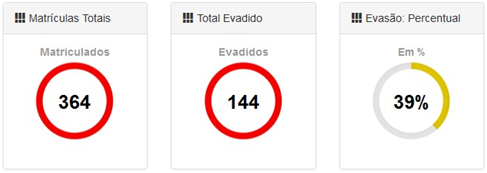
\includegraphics[width=0.7\linewidth]{pip-artigo09-02}
	\caption{Relação de Matrículas, evasão e percentual de evasão do Campus Calama, 2015}
	\label{fig:pip-artigo09-02}
\end{figure}

	Do total evadido, o curso Técnico de Informática Integrado ao Ensino Médio contribuiu com 36 desistências, o que equivale a 25\% do total.
	
	São vários os fatores apontados pelos estudantes para justificar a evasão: dificuldades financeiras (40\%), que se relacionam com a necessidade de trabalhar, dificuldades de aprendizagem (10\%), grande quantidade de componentes curriculares a serem cursadas e de provas e trabalhos que se acumulam (43\%), falta de identificação com o curso (03\%), falta de apoio institucional (07\%). Especialistas apontam, que a evasão escolar é produto da interação de vários fatores, dentre eles, os psicológicos: referentes a fatores cognitivos e psicoemocionais dos alunos (BRASIL, 2006), socioculturais: relativos ao contexto social do aluno e as características familiares (OLIVEIRA, 2001) e os institucionais: como os métodos de ensino, o currículo e o acompanhamento pedagógico (AQUINO, 1997). Ceratti (2008) e Brasil (2006) destacam ainda que a economia e a política nacional são fatores que também incidem no sucesso ou fracasso escolar e na permanência ou evasão.
	
	\section*{Considerações}

A evasão escolar é um fenômeno complexo, que desafia a educação brasileira desde seus primórdios. Dado seu perfil, é necessário abordá-la a partir de uma pluralidade de percepções, e para combatê-la, uma pluralidade de ações, técnica e intervenções também se faz necessária. À escola cabe, sobretudo,  verificar seus projetos pedagógicos de curso, buscar compreender as dificuldades apresentadas pelos estudantes (tanto pelos que evadiram quanto por aqueles que têm apresentado faltas, baixa participação e baixa motivação), bem como fomentar o debate sobre os macro problemas que incidem no processo, como a insuficiência de recursos para os programas de assistência estudantil, a precarização do ensino perpetrada pelas forças políticas hegemônicas, bem como sobre sua política de inclusão e apoio à permanência, política essa que não deve se resumir ao repasse financeiro de auxílios, mas englobar um comprometimento multiprofissional com os estudantes e os desafios que enfrentam.

O curso de Informática do IFRO necessita ser analisado com essa mesma postura, e conforme indicação dos entrevistados, necessita corrigir a distorção entre teoria e prática, de modo a tornar o currículo mais lógico e integrador.

	
	\section*{Instituição de Fomento}
	
	FAPERO
	
	\section*{Referências}
	
	\sloppy
	
	\noindent AQUINO, J. G. O mal-estar na escola contemporânea: erro e fracasso em questão. In: \_\_\_\_\_. (Org.). Erro e fracasso na escola: alternativas teóricas e práticas. 4. ed. São Paulo: Summus,1997, p.91-110.
	
	\noindent BRASIL. Ministério da Educação. Secretaria da Educação Continuada,Alfabetização e Diversidade. Alunas e alunos da EJA. Brasília: Coleção: Trabalhando com a Educação de Jovens e Adultos,2006.
		
	\noindent \_\_\_\_\_. República Federativa do Brasil. Constituição Federal.1988.
	
	\noindent \_\_\_\_\_. República Federativa do Brasil Lei 9394 de 20 de dezembro de1996.
	
	\noindent CERATTI, M. R. N. Evasão escolar: causas e conseqüências. 2008. Disponível em:
	<http://www.see.go.gov.br/imprensa/documentos/arquivos/15\%20-
	\%20Manual\%20de\%20Gest\%C3\%A3o\%20Pedag\%C3\%B3gico\%20e\%20Administra tivo/2.10\%20Combate\%20\%C3\%A0\%20evas\%C3\%A3o/EVAS\%C3\%83O\%20ESC OLAR\%20-\%20CAUSAS\%20E\%20CONSEQU\%C3\%8ANCIAS.pdf>. Acesso em: 19
	set. 2016.
	
	\noindent FREITAG, B. Escola, Estado e Sociedade. São Paulo: Moraes, 1980.
	
	\noindent OLIVEIRA, M. K. de. Jovens e adultos como sujeitos de conhecimento e aprendizagem. In: RIBEIRO, V. M. (Org.). Educação de Jovens e Adultos: novos leitores, novas leituras. São Paulo: Ação Educativa; Campinas: Mercado das Letras, 2001, p. 15-44.
	
\end{document}